\documentclass[12pt]{article}
\usepackage[paper=letterpaper,margin=2cm]{geometry}
\usepackage{amsmath,amssymb,amsfonts}
\usepackage{newtxtext,newtxmath}
\usepackage{enumitem}
\usepackage{titling}
\usepackage{subfig,graphicx}
\usepackage[colorlinks=true]{hyperref}
\usepackage{multirow}
\usepackage{listings}
\usepackage[dvipsnames]{xcolor}
\usepackage{float}

\definecolor{codegreen}{rgb}{0,0.6,0}
\definecolor{codegray}{rgb}{0.5,0.5,0.5}
\definecolor{codepurple}{rgb}{0.58,0,0.82}

% BACKGROUND BOX COLORS
\definecolor{bblue}{HTML}{7cc0f3}
\definecolor{bgreen}{HTML}{84b082}
\definecolor{bred}{HTML}{f6908e}
\definecolor{byellow}{HTML}{e0b400}
\definecolor{bmint}{HTML}{00c49a}

% \highlight[<colour>]{<stuff>}
\newcommand{\highlight}[2][yellow]{\mathchoice
  {\colorbox{#1}{$\displaystyle#2$}}
  {\colorbox{#1}{$\textstyle#2$}}
  {\colorbox{#1}{$\scriptstyle#2$}}
  {\colorbox{#1}{$\scriptscriptstyle#2$}}}

\lstdefinestyle{mystyle}{
    commentstyle=\color{codegreen},
    keywordstyle=\color{magenta},
    numberstyle=\tiny\color{codegray},
    stringstyle=\color{codepurple},
    basicstyle=\ttfamily\footnotesize,
    breakatwhitespace=false,
    breaklines=true,
    captionpos=b,
    keepspaces=true,
    numbers=left,
    numbersep=6pt,
    showspaces=false,
    showstringspaces=false,
    showtabs=false,
    tabsize=2
}
\lstset{style=mystyle}

\begin{document}
\begin{center}
\large{Aprendizagem 2023} \\
Homework III -- Group 28 \\
\vskip 0.3cm
Gonçalo Bárias (ist1103124) \& Raquel Braunschweig (ist1102624)\vskip 1cm

\large{\textbf{Part I}: Pen and Paper}\normalsize
\end{center}

\noindent For questions in this group, show your numerical results with 5 decimals or scientific notation. \\
\textit{Hint}: we highly recommend the use of \texttt{numpy} (e.g., \texttt{linalg.pinv} for inverse) or other programmatic
facilities to support the calculus involved in both questions (1) and (2).

\begin{enumerate}[leftmargin=\labelsep]
    \item \textbf{Consider the problem of learning a regression model from 4 bivariate observations} \\

          \vskip -0.2cm
          \textbf{$\left\{\begin{pmatrix} 0.7 \\ -0.3 \end{pmatrix}, \begin{pmatrix} 0.4 \\ 0.5 \end{pmatrix}, \begin{pmatrix} -0.2 \\ 0.8 \end{pmatrix},
          \begin{pmatrix} -0.4 \\ 0.3 \end{pmatrix}\right\}$ with targets $(0.8, 0.6, 0.3, 0.3)$.}

    \begin{enumerate}
        \item \textbf{Given the radial basis function, $\phi_j(x) = \text{exp}\left({ -\frac{\| \mathbf{x} - \boldsymbol{c}_j \|^2}{2} }\right)$ that transforms
              the original space onto a new space characterized by the similarity of the original observations to the following data points
              $\left\{ c_1 = \begin{bmatrix} 0 & 0 \\ \end{bmatrix}^T,\, c_2 = \begin{bmatrix} 1 & -1 \\ \end{bmatrix}^T,\, c_3 = \begin{bmatrix} -1 & 1 \\ \end{bmatrix}^T\right\}$. \\
              Learn the Ridge regression ($l_2$ regularization) using the closed solution with $\lambda = 0.1$.}

              \vskip 0.3cm
              \textbf{Note:} The intermediate values and matrices, in both items of this exercise, show values rounded to 5 decimal places,
              but all intermediate calculations have been carried out without rounding. The values were obtained with the help of \texttt{numpy}
              as suggested in the prompt. The code can be found in the Jupyter notebook \texttt{G028.ipynb}.

              Considering the data points along with the 4 bivariate observations, we can calculate the values of $\phi_1(x), \phi_2(x)$
              and $\phi_3(x)$ for each observation, with $\phi_0(x)$ always being equal to 1.

              \begin{center}
                  \captionsetup{type=table}
                  \begin{tabular}{c|cccc}
                      $x$           & $\phi_0(x)$ & $\phi_1(x)$ & $\phi_2(x)$ & $\phi_3(x)$ \\
                      \hline
                      $(0.7, -0.3)$ & 1           & 0.74826     & 0.74826     & 0.10127     \\
                      $(0.4, 0.5)$  & 1           & 0.81465     & 0.27117     & 0.33121     \\
                      $(-0.2, 0.8)$ & 1           & 0.71177     & 0.09633     & 0.71177     \\
                      $(-0.4, 0.3)$ & 1           & 0.88250     & 0.16122     & 0.65377
                  \end{tabular}
                  \captionof{table}{Value of $\phi_j(x)$ for each observation, $j=0,\dots,3$}
                  \label{ex1a-phi-table}
              \end{center}

              Our goal is to perform a regression where the prediction is given by:
              \begin{equation}\label{ex1a-z-hat}
                  \hat{z}(x, w)
                  = \highlight[bblue]{w_0}\phi_0(x) +
                  \highlight[bred]{w_1}\phi_1(x) +
                  \highlight[bgreen]{w_2}\phi_2(x) +
                  \highlight[byellow]{w_3}\phi_3(x)
              \end{equation}

              Since we want to learn a Ridge regression model, we will need to minimize the following regularized least-squares estimator:
              \begin{equation}\label{ex1a-least-squares}
                  E(w) = \frac{1}{2} \sum_{i = 1}^{N} (z_i - w^T \cdot x_i)^2 + \frac{\lambda}{2} \| w \|_{2}^2
              \end{equation}

              To minimize \eqref{ex1a-least-squares}, we set its gradient equal to 0 and obtain the closed-form solution with $\lambda = 0.1$ in equation \eqref{ex1a-ridge}.
              In the equation, we have that $\Phi$ is the matrix after applying $\phi_j(x)$ to the observations (Table \ref{ex1a-phi-table}) and $z$ is the vector
              of targets for the observations, $z = \begin{bmatrix}0.8 & 0.6 & 0.3 & 0.3\end{bmatrix}^T$.

              \vskip -0.2cm
              \begin{equation}\label{ex1a-ridge}
                  \nabla E(w) = 0 \;\Leftrightarrow\; w = \left(\Phi^T \Phi + \lambda I\right)^{-1} \cdot \Phi^T z
                  \;\Leftrightarrow\; w = \left(\Phi^T \Phi + 0.1 I\right)^{-1} \cdot \Phi^T z
              \end{equation}

              \vskip -0.2cm
              $$
                  \Phi = \begin{bmatrix}
                      1.00000 & 0.74826 & 0.74826 & 0.10127 \\
                      1.00000 & 0.81465 & 0.27117 & 0.33121 \\
                      1.00000 & 0.71177 & 0.09633 & 0.71177 \\
                      1.00000 & 0.88250 & 0.16122 & 0.65377
                  \end{bmatrix}
                  \quad
                  \quad
                  \Phi^T = \begin{bmatrix}
                      1.00000 & 1.00000 & 1.00000 & 1.00000 \\
                      0.74826 & 0.81465 & 0.71177 & 0.88250 \\
                      0.74826 & 0.27117 & 0.09633 & 0.16122 \\
                      0.10127 & 0.33121 & 0.71177 & 0.65377
                  \end{bmatrix}
              $$

              \textbf{Therefore}, we can then calculate the remaining values, until we get the vector $w$:

              $$
                  \begin{aligned}
                      \Phi^T \Phi                                          & = \begin{bmatrix}
                                                                                   4.00000 & 3.15718 & 1.27698 & 1.79802 \\
                                                                                   3.15718 & 2.50897 & 0.99165 & 1.42916 \\
                                                                                   1.27698 & 0.99165 & 0.66870 & 0.33955 \\
                                                                                   1.79802 & 1.42917 & 0.33956 & 1.05399
                                                                               \end{bmatrix}                                                            \\
                      \Phi^T \Phi + \highlight[bmint]{0.1} I               & = \begin{bmatrix}
                                                                                  \highlight[bmint]{4.10000}  & 3.15718 & 1.27698 & 1.79802 \\
                                                                                   3.15718 & \highlight[bmint]{2.60897} & 0.99165 & 1.42917 \\
                                                                                   1.27698 & 0.99165 & \highlight[bmint]{0.76870} & 0.33956 \\
                                                                                   1.79802 & 1.42917 & 0.33956 & \highlight[bmint]{1.15399}
                                                                               \end{bmatrix}                                                            \\
                      \left(\Phi^T \Phi + 0.1 I\right) ^ {-1}              & = \begin{bmatrix}
                                                                                   4.54826  & -3.77682 & -1.86117 & -1.86155 \\
                                                                                   -3.77682 & 5.98285  & -0.88543 & -1.26432 \\
                                                                                   -1.86117 & -0.88543 & 4.33276  & 2.72156  \\
                                                                                   -1.86155 & -1.26432 & 2.72156  & 4.53204
                                                                               \end{bmatrix}                                                            \\
                      \left(\Phi^T \Phi + 0.1 I\right) ^ {-1} \cdot \Phi^T & = \begin{bmatrix}
                                                                                   0.14105  & 0.35022  & 0.35575  & -0.30185 \\
                                                                                   -0.09064 & 0.43823  & -0.50361 & 0.53370  \\
                                                                                   0.99394  & -0.50615 & -0.13690 & -0.16477 \\
                                                                                   -0.31222 & -0.65246 & 0.72647  & 0.42436
                                                                               \end{bmatrix}                                                            \\
                      w = \left(\Phi^T \Phi + 0.1 I\right) ^ {-1} \cdot \Phi^T z & = \begin{bmatrix}
                                                                                         \highlight[bblue]{0.33914} & \highlight[bred]{0.19945} &
                                                                                         \highlight[bgreen]{0.40096} & \highlight[byellow]{-0.29600}
                                                                                     \end{bmatrix}^T
                  \end{aligned}
              $$

              Having calculated the vector $w$, we now know the values of each weight in the regression:

              $$
                  \begin{array}{cccc}
                      \highlight[bblue]{w_0 = 0.33914}  &
                      \highlight[bred]{w_1 = 0.19945}   &
                      \highlight[bgreen]{w_2 = 0.40096} &
                      \highlight[byellow]{w_3 = -0.29600}
                  \end{array}
              $$

              \textbf{Finally}, replacing them in \eqref{ex1a-z-hat} gives us the regression expression:

              \begin{equation}\label{ex1a-final-z-hat}
                  \hat{z}(x, w)
                  = 0.33914 + 0.19945\,\phi_1(x) +
                  0.40096\,\phi_2(x) - 0.29600\,\phi_3(x)
              \end{equation}

        \item \textbf{Compute the training RMSE for the learnt regression.}

              \vskip 0.3cm
              The RMSE (Root Mean Square Error) is given by:

              \begin{equation}\label{ex1b-rmse}
                  \text{RMSE} = \sqrt{\frac{1}{N} \sum_{i = 1}^{N} (z_i - \hat{z}_i)^2}
              \end{equation}

              Here we have $N = 4$, because 4 is the number of samples in the dataset, $z_i$ is the true label for the $i$-th sample and $\hat{z}_i$
              is the predicted label for the $i$-th sample.

              Using \eqref{ex1a-final-z-hat} from the previous item, we can determine $\hat{z}$ for the 4 observations:

              $$
                \Phi = \begin{bmatrix}
                      1.00000 & 0.74826 & 0.74826 & 0.10127 \\
                      1.00000 & 0.81465 & 0.27117 & 0.33121 \\
                      1.00000 & 0.71177 & 0.09633 & 0.71177 \\
                      1.00000 & 0.88250 & 0.16122 & 0.65377
                    \end{bmatrix} \,
                \land \,
                w = \begin{bmatrix}{}
                      \highlight[bblue]{0.33914}  \\
                      \highlight[bred]{0.19945}   \\
                      \highlight[bgreen]{0.40096} \\
                      \highlight[byellow]{-0.29600}
                    \end{bmatrix} \,
               \Rightarrow \,
               \hat{z} = \Phi w = \begin{bmatrix}{}
                                   0.75844 \\
                                   0.51232 \\
                                   0.30905 \\
                                   0.38629
                               \end{bmatrix}
              $$

              \textbf{Finally}, we can take $z = \begin{bmatrix}0.8 & 0.6 & 0.3 & 0.3\end{bmatrix}^T$ along with $\hat{z}$ and calculate RMSE, using \eqref{ex1b-rmse}:
              $$
                  \text{RMSE} = \sqrt{\frac{1}{4} \times \sum_{i = 1}^{4} (z_i - \hat{z}_i)^2} = \sqrt{\frac{1}{4} \times 0.01694} = \mathbf{0.06508}
              $$
    \end{enumerate}

    \item \textbf{Consider a MLP classifier of three outcomes - A, B and C - characterized by the following weights and activation function for every unit:} \\

          \begin{center}
              \vskip -0.3cm
              $\text{W}^{[1]} = \begin{bmatrix} 1 & 1 & 1 & 1 \\ 1 & 1 & 2 & 1 \\ 1 & 1 & 1 & 1\end{bmatrix},\; \text{b}^{[1]} = \begin{bmatrix} 1 \\ 1 \\ 1 \end{bmatrix},\;
              \text{W}^{[2]} = \begin{bmatrix} 1 & 4 & 1 \\ 1 & 1 & 1 \end{bmatrix},\; \text{b}^{[2]} = \begin{bmatrix} 1 \\ 1 \end{bmatrix},\;
              \text{W}^{[3]} = \begin{bmatrix} 1 & 1 \\ 3 & 1 \\ 1 & 1\end{bmatrix},\; \text{b}^{[3]} = \begin{bmatrix} 1 \\ 1 \\ 1 \end{bmatrix}$ \\
          \end{center}

          \[ f\left(x\right) = \frac{{e^{0.5x - 2} - e^{-0.5x + 2}}}{{e^{0.5x - 2} + e^{-0.5x + 2}}} = \tanh\left(0.5x - 2\right) \] \\

          \vskip -0.5cm
          \textbf{We also have the squared error loss $\frac{1}{2} \|\mathbf{z} - \hat{\mathbf{z}}\|^{2}_{2}$. Perform one batch gradient descent update (with learning rate $\eta = 0.1$) for training
          obvervations $x_1 = \begin{bmatrix} 1 & 1 & 1 & 1 \\ \end{bmatrix}^T$ and $x_2 = \begin{bmatrix} 1 & 0 & 0 & -1 \\ \end{bmatrix}^T$ with targets B and A,
          respectively.}

          \vskip 0.3cm
          \textbf{Note:} To help with the calculations and as suggested in the prompt, we used \texttt{numpy}.
          The code can be found in the Jupyter notebook \texttt{G028.ipynb}.

          To begin, we initiate the process with the \textbf{forward propagation}. Below are the key equations to calculate the values of each
          layer, $x^{[p]}_i$, per observation:

          \vskip -0.2cm
          \begin{align*}
              z^{[p]}_i = W^{[p]} \, x^{[p-1]}_i + b^{[p]} & \qquad\qquad
              x^{[p]}_i = f\left(z^{[p]}_i\right)
          \end{align*}

          The function $f$ is the activation function, for every layer, provided in the prompt, $f\left(z^{[p]}_i\right) = \text{tanh}\left(0.5\,z^{[p]} - 2\right)$.
          In this notation, the value $p$ is the index of the MLP layer and $n$ is the number of the observation, either 1 or 2.

          We can now calculate the values of each node in the multi-layer perceptron with the initialized weights and biases provided in the prompt,
          for each of the observations.

          We will \textbf{start} with $x_1$:
            \begingroup
            \allowdisplaybreaks
            \begin{align*}
                z^{[1]}_1 &= {W}^{[1]} \, {x}^{[0]}_1 + {b}^{[1]} = \begin{bmatrix} 1 & 1 & 1 & 1 \\ 1 & 1 & 2 & 1 \\ 1 & 1 & 1 & 1\end{bmatrix} \,  \begin{bmatrix} 1 \\ 1 \\ 1 \\ 1 \end{bmatrix} +
                \begin{bmatrix} 1 \\ 1 \\ 1\end{bmatrix} = \begin{bmatrix} 5 \\ 6 \\ 5\end{bmatrix} \\
                    {x}^{[1]}_1 &= f\left({z}^{[1]}_1\right) = \text{tanh}\left(0.5\,{z}^{[1]}_1 - 2\right) \approx \begin{bmatrix} 0.46212 \\ 0.76159 \\ 0.46212\end{bmatrix} \\
                z^{[2]}_1 &= {W}^{[2]} \, {x}^{[1]}_1 + {b}^{[2]} = \begin{bmatrix} 1 & 4 & 1 \\ 1 & 1 & 1\end{bmatrix} \, \begin{bmatrix} 0.46212 \\ 0.76159 \\ 0.46212 \end{bmatrix} +
                \begin{bmatrix} 1 \\ 1\end{bmatrix} \approx \begin{bmatrix} 4.97061 \\ 2.68583\end{bmatrix} \\
                {x}^{[2]}_1 &= f\left({z}^{[2]}_1\right) = \text{tanh}\left(0.5\,{z}^{[2]}_1 - 2\right) \approx \begin{bmatrix} 0.45048 \\ -0.57642\end{bmatrix} \\
                z^{[3]}_1 &= {W}^{[3]} \, {x}^{[2]}_1 + {b}^{[3]} = \begin{bmatrix} 1 & 1 \\ 3 & 1 \\ 1 & 1\end{bmatrix} \,  \begin{bmatrix} 0.45048 \\ -0.57642\end{bmatrix} +
                \begin{bmatrix} 1 \\ 1 \\ 1\end{bmatrix} \approx \begin{bmatrix} 0.87406 \\ 1.77503 \\ 0.87406\end{bmatrix} \\
                {x}^{[3]}_1 &= f\left({z}^{[3]}_1\right) = \text{tanh}\left(0.5\,{z}^{[3]}_1 - 2\right) \approx \begin{bmatrix} -0.9159 \\ -0.80494 \\ -0.9159\end{bmatrix}
            \end{align*}
            \endgroup

          \vskip -0.2cm
          \textbf{Next} in line is $x_2$:
            \begingroup
            \allowdisplaybreaks
            \begin{align*}
                z^{[1]}_2 &= {W}^{[1]} \, {x}^{[0]}_2 + {b}^{[1]} = \begin{bmatrix} 1 & 1 & 1 & 1 \\ 1 & 1 & 2 & 1 \\ 1 & 1 & 1 & 1\end{bmatrix} \,  \begin{bmatrix} 1 \\ 0 \\ 0 \\ -1 \end{bmatrix} +
                \begin{bmatrix} 1 \\ 1 \\ 1\end{bmatrix} = \begin{bmatrix} 1 \\ 1 \\ 1\end{bmatrix} \\
                {x}^{[1]}_2 &= f\left({z}^{[1]}_2\right) = \text{tanh}\left(0.5\,{z}^{[1]}_2 - 2\right) \approx \begin{bmatrix} -0.90515 \\ -0.90515 \\ -0.90515\end{bmatrix} \\
                z^{[2]}_2 &= {W}^{[2]} \, {x}^{[1]}_2 + {b}^{[2]} = \begin{bmatrix} 1 & 4 & 1 \\ 1 & 1 & 1\end{bmatrix} \,  \begin{bmatrix} -0.90515 \\ -0.90515 \\ -0.90515 \end{bmatrix} +
                \begin{bmatrix} 1 \\ 1\end{bmatrix} \approx \begin{bmatrix} -4.43089 \\ -1.71544\end{bmatrix} \\
                {x}^{[2]}_2 &= f\left({z}^{[2]}_2\right) = \text{tanh}\left(0.5\,{z}^{[2]}_2 - 2\right) \approx \begin{bmatrix} -0.99956 \\ -0.99343\end{bmatrix} \\
                z^{[3]}_2 &= {W}^{[3]} \, {x}^{[2]}_2 + {b}^{[3]} = \begin{bmatrix} 1 & 1 \\ 3 & 1 \\ 1 & 1\end{bmatrix} \,  \begin{bmatrix} -0.99956 \\ -0.99343\end{bmatrix} +
                \begin{bmatrix} 1 \\ 1 \\ 1\end{bmatrix} \approx \begin{bmatrix} -0.993 \\ -2.99212 \\ -0.993\end{bmatrix} \\
                {x}^{[3]}_2 &= f\left({z}^{[3]}_2\right) = \text{tanh}\left(0.5\,{z}^{[3]}_2 - 2\right) \approx \begin{bmatrix} -0.98652 \\ -0.99816 \\ -0.98652\end{bmatrix}
            \end{align*}
            \endgroup

          Now that we have obtained the values for our observations, considering the initial weights and biases, we can initiate the \textbf{back propagation} process
          to perform a batch gradient descent update (with learning rate $\eta = 0.1$).

          The updated values for the weights and biases can be obtained by the following equations:

          \begin{equation}\label{ex2-new-weight}
              W^{[i]}_{new} = W^{[i]}_{old} + \Delta W^{[i]} = W^{[i]}_{old} - \eta \frac{\partial E}{\partial W^{[i]}} = W^{[i]}_{old} - 0.1 \frac{\partial E}{\partial W^{[i]}}
          \end{equation}

          \begin{equation}\label{ex2-new-bias}
              b^{[i]}_{new} = b^{[i]}_{old} + \Delta b^{[i]} = b^{[i]}_{old} - \eta \frac{\partial E}{\partial b^{[i]}} = b^{[i]}_{old} - 0.1 \frac{\partial E}{\partial b^{[i]}}
          \end{equation}

          We first need to take into account the loss function, which, as per the prompt, is the half squared error loss, defined as follows:

          \vskip -0.3cm
          \begin{equation*}
              E(w) = \frac{1}{2} \|\mathbf{z} - \hat{\mathbf{z}}\|^{2}_{2}
          \end{equation*}

          The next step involves computing its derivatives by applying the \textbf{chain rule}:

          \begin{equation*}
            \frac{\partial E}{\partial W^{[p]}} = \sum_{i=1}^{2} \left(\frac{\partial E}{\partial x^{[p]}_i} \circ
              \frac{\partial x^{[p]}_i}{\partial z^{[p]}_i} \cdot \frac{\partial z^{[p]}_i}{\partial W^{[p]}} \right)
            \qquad
            \frac{\partial E}{\partial b^{[p]}} = \sum_{i=1}^{2} \left(\frac{\partial E}{\partial x^{[p]}_i} \circ
              \frac{\partial x^{[p]}_i}{\partial z^{[p]}_i} \cdot \frac{\partial z^{[p]}_i}{\partial b^{[p]}} \right)
          \end{equation*}

          This can be broken down into:

          \vskip -0.3cm
          \begin{equation*}
              \frac{\partial E}{\partial x^{[p]}_i} \circ \frac{\partial x^{[p]}_i}{\partial z^{[p]}_i} = \delta^{[p]}_i
          \end{equation*}

          \begin{equation*}
              \frac{\partial E}{\partial x^{[3]}_i} = \frac{1}{2} \times 2 \times \left(x^{[3]}_i - t_i\right)
              = x^{[3]}_i - t_i
          \end{equation*}

          \begin{equation*}
              \frac{\partial E}{\partial x^{[p]}_i} = \frac{\partial z^{[p+1]}_i}{\partial x^{[p]}_i} \cdot
              \underbrace{\frac{\partial x^{[p+1]}_i}{\partial z^{[p+1]}_i} \circ \frac{\partial E}{\partial x^{[p+1]}_i}}_{\delta^{[p+1]}_i}
              = \left(W^{[p+1]}\right)^{T} \cdot \delta^{[p+1]}_i, \;\; p \neq 3 \quad \text{(using recursion)}
          \end{equation*}

          \vskip -0.5cm
          \begin{align*}
              \frac{\partial x^{[p]}_i}{\partial z^{[p]}_i} & = f'\left(z^{[p]}_i\right) = \text{tanh}'\left(0.5 \times z^{[p]}_i - 2\right) \times
              \frac{d}{d z^{[p]}_i} \left(0.5 \times z^{[p]}_i - 2\right) \\
              & = \text{sech}^2\left(0.5 \times z^{[p]}_i - 2\right) \times 0.5
          \end{align*}

          \begin{equation*}
              \frac{\partial z^{[p]}_i}{\partial W^{[p]}} = \left(x^{[p-1]}_i\right)^{T} \qquad\qquad
              \frac{\partial z^{[p]}_i}{\partial b^{[p]}} = 1
          \end{equation*}

          \textbf{Therefore,} the derivatives of the loss function are given by:

          \begin{equation}\label{ex2-derivate-loss-smiplified}
            \frac{\partial E}{\partial W^{[p]}} = \sum_{i=1}^{2} \left(\delta^{[p]}_i \cdot \left(x^{[p-1]}_i\right)^{T} \right) \qquad\qquad
            \frac{\partial E}{\partial b^{[p]}} = \sum_{i=1}^{2} \left(\delta^{[p]}_i\right)
          \end{equation}

          When computing \(\delta\), we split it into two separate cases: if it is in  last layer \eqref{ex2-deltalastlayer} for $p = 3$, or in non-external
          layers \eqref{ex2-deltanotlastlayer} for any $p \neq 3$:

          \begin{equation}\label{ex2-deltalastlayer}
              \delta^{[3]}_i = \left(x^{[3]}_i - t_i\right) \circ \text{sech}^{2}\left(0.5 \times z^{[3]}_i - 2\right) \times 0.5
          \end{equation}

          \begin{equation}\label{ex2-deltanotlastlayer}
              \delta^{[p]}_i = \left(\left(W^{[p+1]}\right)^{T} \cdot \delta^{[p+1]}_i\right) \circ \text{sech}^{2}\left(0.5 \times z^{[p]}_i - 2\right) \times 0.5, \;\; p \neq 3
          \end{equation}

          \textbf{Since,} the \texttt{tanh} function has a codomain in $[-1,1]$ and since the targets for $x_1$ and $x_2$ are B and A, respectively, we can
          conclude the following encodings for the outputs:

          \begin{equation*}
              t_1 = \begin{bmatrix} -1 & 1 & -1\end{bmatrix}^T \qquad\qquad
              t_2 = \begin{bmatrix} 1 & -1 & -1\end{bmatrix}^T
          \end{equation*}

        \textbf{Now,} we have all we need to compute the values for the deltas, $\delta$, by replacing the equation on \eqref{ex2-deltalastlayer} for $p=3$,
        and \eqref{ex2-deltanotlastlayer} for any $p \neq 3$:
        \begingroup
        \allowdisplaybreaks
          \begin{align*}
            \delta^{[3]}_1 &= \left(x^{[3]}_1 - t_1\right) \circ  \text{sech}^{2}\left(0.5\times z^{[3]}_1 - 2\right) \times 0.5 =  \\
            &=  \left(\begin{bmatrix} -0.9159 \\ -0.80494 \\ -0.9159\end{bmatrix} - \begin{bmatrix} -1 \\ 1 \\ -1 \end{bmatrix}\right) \circ \text{sech}^{2}\left(0.5\times \begin{bmatrix} 0.87406 \\ 1.77503 \\ 0.87406\end{bmatrix} \times 0.5\right) = \\
            &= \begin{bmatrix} 0.00678 \\ -0.31773 \\ 0.00678 \end{bmatrix} \\
            \delta^{[3]}_2 &= \left(x^{[3]}_2 - t_2\right) \circ  \text{sech}^{2}\left(0.5\times z^{[3]}_2 - 2\right) \times 0.5 =  \\
            &=  \left(\begin{bmatrix} -0.98652 \\ -0.99816 \\ -0.98652\end{bmatrix} - \begin{bmatrix} 1 \\ -1 \\ -1\end{bmatrix}\right) \circ \text{sech}^{2}\left(0.5\times \begin{bmatrix} -0.993 \\ -2.99212 \\ -0.993\end{bmatrix} \times 0.5\right) = \\
            &= \begin{bmatrix} -0.0266 \\ 0 \\ 0.00018 \end{bmatrix}
          \end{align*}
        \endgroup

        \begingroup
        \allowdisplaybreaks
          \begin{align*}
              \delta^{[2]}_1 &= \left(\left(W^{[3]}\right)^{T} \cdot \delta^{[3]}_1\right) \circ \text{sech}^{2}\left(0.5\times z^{[2]}_1 - 2\right) \times 0.5 = \\
             &= \left(\begin{bmatrix} 1 1 \\ 3 1 \\ 1 1\end{bmatrix}^{T} \cdot \begin{bmatrix} 0.00678 \\ -0.31773 \\ 0.00678 \end{bmatrix}\right) \circ \text{sech}^{2}\left(0.5\times\begin{bmatrix} 4.97061 \\ 2.68583\end{bmatrix} - 2\right) \times 0.5 = \\
             &= \begin{bmatrix} -0.37448 \\ -0.10156 \end{bmatrix} \\
                 \delta^{[2]}_2 &= \left(\left(W^{[3]}\right)^{T} \cdot \delta^{[3]}_2\right) \circ  \text{sech}^{2}\left(0.5\times z^{[2]}_2 - 2\right) \times 0.5 = \\
             &= \left(\begin{bmatrix} 1 1 \\ 3 1 \\ 1 1\end{bmatrix}^{T} \cdot \begin{bmatrix} -0.0266 \\ 0 \\ -0.00018 \end{bmatrix}\right) \circ \text{sech}^{2}\left(0.5\times\begin{bmatrix} 4.97061 \\ 2.68583\end{bmatrix} - 2\right) \times 0.5 = \\
             &= \begin{bmatrix} -1 \times 10^{-5} \\ -1.7 \times 10^{-4} \end{bmatrix}
          \end{align*}
        \endgroup

        \begingroup
        \allowdisplaybreaks
          \begin{align*}
              \delta^{[1]}_1 &= \left(\left(W^{[2]}\right)^{T} \cdot \delta^{[2]}_1\right) \circ \text{sech}^{2}\left(0.5 \times z^{[1]}_1 - 2\right) \times 0.5 = \\
             &= \left(\begin{bmatrix} 1 4 1 \\ 1 1 1 \end{bmatrix}^{T} \cdot \begin{bmatrix} -0.37448 \\ -0.10156 \end{bmatrix}\right) \circ \text{sech}^{2}\left(0.5 \times \begin{bmatrix}  5 \\ 6 \\ 5 \end{bmatrix} - 2\right) \times 0.5 = \\
             &= \begin{bmatrix} -0.18719 \\ -0.33587 \\ -0.18719\end{bmatrix} \\
                 \delta^{[1]}_2 &= \left(\left(W^{[2]}\right)^{T} \cdot \delta^{[2]}_2\right) \circ  \text{sech}^{2}\left(0.5\times z^{[1]}_2 - 2\right) \times 0.5 = \\
             &= \left(\begin{bmatrix} 1 4 1 \\ 1 1 1 \end{bmatrix}^{T} \cdot \begin{bmatrix} -1 \times 10^{-5} \\ -1.7 \times 10^{-4} \end{bmatrix}\right) \circ \text{sech}^{2}\left(0.5\times\begin{bmatrix}  1 \\ 1 \\ 1 \end{bmatrix} - 2\right) \times 0.5 = \\
             &= \begin{bmatrix} -2 \times 10^{-5} \\ -2 \times 10^{-5} \\ -2 \times 10^{-5}\end{bmatrix}
          \end{align*}
        \endgroup

        \textbf{Next,} we will compute the derivatives of the loss function, employing the first equation at \eqref{ex2-derivate-loss-smiplified}:
        \begingroup
        \allowdisplaybreaks
          \begin{align*}
            \frac{\partial E}{\partial W^{[1]}} &= \sum_{i=1}^{2} \left(\delta^{[1]}_i \cdot \left(x^{[0]}_i\right)^{T}\right)
             = \left(\delta^{[1]}_1 \cdot \left(x^{[0]}_1\right)^{T}\right) + \left(\delta^{[1]}_2 \cdot \left(x^{[0]}_2\right)^{T}\right) = \\
             &= \left(\begin{bmatrix} -0.18719 \\ -0.33587 \\ -0.18719 \end{bmatrix} \cdot \begin{bmatrix} 1 \\ 1 \\ 1 \\ 1\end{bmatrix}^{T}\right) +
                 \left(\begin{bmatrix} -2 \times 10^{-5} \\ -2 \times 10^{-5} \\ -2 \times 10^{-5}  \end{bmatrix} \cdot \begin{bmatrix} 1 \\ 0 \\ 0 \\ -1\end{bmatrix}^{T}\right) = \\
             &= \begin{bmatrix} -0.18721 & -0.18719 & -0.18719 & -0.18717\\ -0.33589 & -0.33587 & -0.33587 & -0.33585 \\ -0.18721 & -0.18719 & -0.18719 & -0.18717\end{bmatrix} \\
            \frac{\partial E}{\partial W^{[2]}} &= \sum_{i=1}^{2} \left(\delta^{[2]}_i \cdot \left(x^{[1]}_i\right)^{T}\right)
             = \left(\delta^{[2]}_1 \cdot \left(x^{[1]}_1\right)^{T}\right) + \left(\delta^{[2]}_2 \cdot \left(x^{[1]}_2\right)^{T}\right) = \\
             &= \left(\begin{bmatrix} -0.37448 \\ 0.10156 \end{bmatrix} \cdot \begin{bmatrix} 0.46212 \\ 0.76159 \\ 0.46212\end{bmatrix}^{T}\right) +
                 \left(\begin{bmatrix} -1 \times 10^{-5} \\ -1.7 \times 10^{-4}  \end{bmatrix} \cdot \begin{bmatrix} -0.90515 \\ -0.90515 \\ -0.90515\end{bmatrix}^{T}\right) = \\
             &= \begin{bmatrix} -0.17304 & -0.28519 & -0.17304\\ -0.04678 & -0.07719 & -0.04678 \end{bmatrix} \\
            \frac{\partial E}{\partial W^{[3]}} &= \sum_{i=1}^{2} \left(\delta^{[3]}_i \cdot \left(x^{[2]}_i\right)^{T}\right)
             = \left(\delta^{[3]}_1 \cdot \left(x^{[2]}_1\right)^{T}\right) + \left(\delta^{[3]}_2 \cdot \left(x^{[2]}_2\right)^{T}\right) = \\
             &= \left(\begin{bmatrix} 0.00678 \\ -0.31773 \\ 0.00678 \end{bmatrix} \cdot \begin{bmatrix} 0.45048 \\ -0.57642\end{bmatrix}^{T}\right) +
                 \left(\begin{bmatrix} -0.0266 \\ 0 \\ 0.00018 \end{bmatrix} \cdot \begin{bmatrix} -0.99956 \\ -0.99343\end{bmatrix}^{T}\right) = \\
             &= \begin{bmatrix} 0.02964 & 0.02252 \\ -0.14314 & 0.18315 \\ 0.00287 & -0.00408 \end{bmatrix}
          \end{align*}
        \endgroup

        \textbf{Next,} we will employ the second equation at \eqref{ex2-derivate-loss-smiplified}:
        \begingroup
        \allowdisplaybreaks
          \begin{align*}
            \frac{\partial E}{\partial b^{[1]}} &= \sum_{i=1}^{2} \left(\delta^{[1]}_i\right)
             = \delta^{[1]}_1 + \delta^{[1]}_2
             = \begin{bmatrix} -0.18719 \\ -0.33587 \\ -0.18719 \end{bmatrix} +
                 \begin{bmatrix} -2 \times 10^{-5} \\ -2 \times 10^{-5} \\ -2 \times 10^{-5} \end{bmatrix}
             = \begin{bmatrix} -0.18721 \\ -0.33589 \\ -0.18721 \end{bmatrix} \\
            \frac{\partial E}{\partial b^{[2]}} &= \sum_{i=1}^{2} \left(\delta^{[2]}_i\right)
             = \delta^{[2]}_1 + \delta^{[2]}_2
             = \begin{bmatrix} -0.37448 \\ 0.10156 \end{bmatrix} +
                 \begin{bmatrix} -1 \times 10^{-5} \\ -1.7 \times 10^{-4}  \end{bmatrix}
             = \begin{bmatrix} -0.37449 \\ -0.10173 \end{bmatrix} \\
            \frac{\partial E}{\partial b^{[3]}} &= \sum_{i=1}^{2} \left(\delta^{[3]}_i\right)
             = \delta^{[3]}_1 + \delta^{[3]}_2
             = \begin{bmatrix} 0.00678 \\ -0.31773 \\ 0.00678 \end{bmatrix} +
                 \begin{bmatrix} -0.0266 \\ 0 \\ 0.00018 \end{bmatrix}
             = \begin{bmatrix} -0.01982 \\ -0.31773 \\ 0.00696 \end{bmatrix}
          \end{align*}
        \endgroup

          \textbf{The final step} is to calculate the updated weights and biases.

          \textbf{By substituting} the values into \eqref{ex2-new-weight}, we obtain the following updated weights:

          \vskip -0.2cm
          \begin{align*}
              W^{[1]}_{new} = & \begin{bmatrix} 1 & 1 & 1 & 1 \\ 1 & 1 & 2 & 1 \\ 1 & 1 & 1 & 1\end{bmatrix}
                - 0.1 \begin{bmatrix} -0.18721 & -0.18719 & -0.18719 & -0.18717 \\ -0.33589 & -0.33587 & -0.33587 & -0.33585 \\ -0.18721 & -0.18719 & -0.18719 & -0.18717 \end{bmatrix} = \\
                = & \begin{bmatrix} 1.01872 & 1.01872 & 1.01872 & 1.01872 \\ 1.03359 & 1.03359 & 2.03359 & 1.03359 \\ 1.01872 & 1.01872 & 1.01872 & 1.01872 \end{bmatrix} \\
              W^{[2]}_{new} = & \begin{bmatrix} 1 & 4 & 1 \\ 1 & 1 & 1 \end{bmatrix} -
                0.1 \begin{bmatrix} -0.17304 & -0.28519 & -0.17304\\ -0.04678 & -0.07719 & -0.04678 \end{bmatrix} = \\
                = & \begin{bmatrix} 1.0173 & 4.02852 & 1.0173 \\ 1.00468 & 1.00772 & 1.00468\end{bmatrix} \\
              W^{[3]}_{new} = & \begin{bmatrix} 1 & 1 \\ 3 & 1 \\ 1 & 1 \end{bmatrix} -
                0.1 \begin{bmatrix}  0.02964 & 0.02252 \\ -0.14314 & 0.18315 \\ 0.00287 & -0.00408 \end{bmatrix} = \\
                = & \begin{bmatrix} 0.99704 & 0.99775 \\ 3.01431 & 0.98169 \\ 0.99971 & 1.00041\end{bmatrix}
          \end{align*}

          \textbf{Finally,} by replacing the values into \eqref{ex2-new-bias}, we get the following updated biases:

          \vskip -0.2cm
          \begin{align*}
              b^{[1]}_{new} &= \begin{bmatrix} 1 \\ 1 \\ 1 \end{bmatrix} - 0.1 \begin{bmatrix} -0.18721 \\ -0.33589 \\ -0.18721\end{bmatrix}
                  = \begin{bmatrix} 1.01872 \\ 1.03359 \\ 1.01872\end{bmatrix} \\
              b^{[2]}_{new} &= \begin{bmatrix} 1\\ 1\end{bmatrix} - 0.1 \begin{bmatrix} -0.37449 \\ -0.10173\end{bmatrix}
                  = \begin{bmatrix} 1.03745 \\ 1.01017\end{bmatrix} \\
              b^{[3]}_{new} &= \begin{bmatrix} 1 \\ 1 \\ 1\end{bmatrix} - 0.1 \begin{bmatrix} -0.01982 \\ -0.31773 \\ 0.00696\end{bmatrix}
                  = \begin{bmatrix} 1.00198 \\ 1.03177 \\ 0.9993\end{bmatrix}
          \end{align*}
\end{enumerate}

\pagebreak

\begin{center}
\large{\textbf{Part II}: Programming and critical analysis}\normalsize
\end{center}

\noindent Considering the \texttt{winequality-red.csv} dataset (available at the webpage) where the goal is  to estimate the quality (sensory appreciation)
of a wine based on physicochemical inputs.

\vskip 0.2cm

\noindent Using a 80-20 training-test split with a fixed seed (\texttt{random\_state=0}), you are asked to learn MLP
regressors to answer the following questions.

\vskip 0.2cm

\noindent Given their stochastic behavior, average the performance of each MLP from 10 runs (for reproducibility consider seeding the MLPs with
\texttt{random\_state $\in$ \{1..10\}}).

\begin{enumerate}[leftmargin=\labelsep]
    \item \textbf{Learn a MLP regressor with 2 hidden layers of size 10, rectifier linear unit activation
          on all nodes, and early stopping with 20\% of training data set aside for validation. All
          remaining parameters (e.g., loss, batch size, regularization term, solver) should be set as
          default. Plot the distribution of the residues (in absolute value) using a histogram.}

          \vskip 0.3cm
          \lstinputlisting[language=Python]{./assets/code_1.py}

          The residues were calculated as the absolute difference between the predicted value and the expected value, for each observation.
          Due to the stochastic behavior of MLP regressors, we took the results of the MLP from 10 runs.

          \begin{figure}[H]
              \centering
              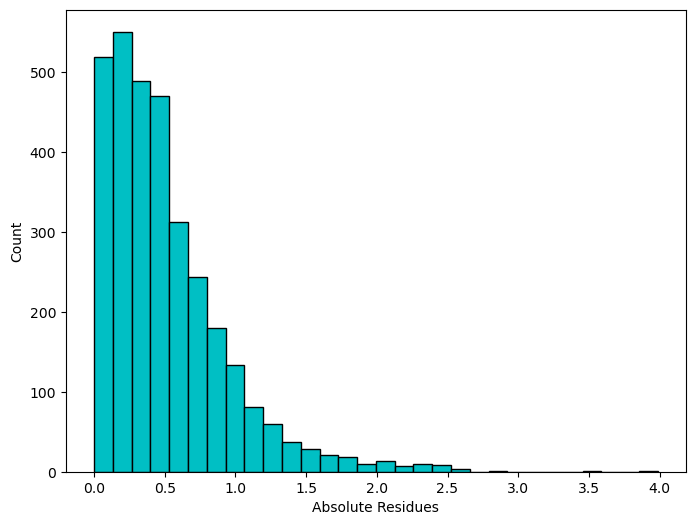
\includegraphics[width=14cm]{./assets/residues_histogram_ex1_PartII.png}
              \caption{The distribution of absolute residues for MLP regression on wine quality prediction using an histogram with 30 bins}
              \label{fig:PartII-ex1}
          \end{figure}

    \item \textbf{Since we are in the presence of a \textit{integer regression} task, a recommended trick is to
          round and bound estimates. Assess the impact of these operations on the MAE of the MLP learnt in the previous question.}

          \vskip 0.3cm
          \lstinputlisting[language=Python]{./assets/code_2.py}

          MAE without operations: 0.5097171955009515 \\
          MAE with rounded and bounded predictions: 0.43875

          \vskip 0.2cm
          By rounding to the nearest unit and bounding the estimates between 1 and 10 (as per the \textit{FAQ}), we get a lower Mean Absolute Error.
          The wine quality is an integer between 1 and 10, so it is expected that rounding and bounding the estimates gets them closer to the real integer values.

    \item \textbf{Similarly assess the impact on RMSE from replacing early stopping by a well-defined
          number of iterations in $\{20,50,100,200\}$ (where one iteration corresponds to a batch).}

          \vskip 0.3cm
          \lstinputlisting[language=Python]{./assets/code_3.py}

          RMSE with 20 iterations: 1.4039789509925442  \\
          RMSE with 50 iterations: 0.7996073631460567  \\
          RMSE with 100 iterations: 0.6940361469112144 \\
          RMSE with 200 iterations: 0.6554543932216472

    \item \textbf{Critically comment the results obtained in the previous question, hypothesizing at least
          one reason why early stopping favors and/or worsens performance.}

          \vskip 0.3cm
          Increasing the number of iterations consistently lowered the Root Mean Squared Error (RMSE).
          This outcome is expected since additional iterations provide the model with more opportunities to adjust its weights and biases, potentially
           leading to a more precise fit to the data.

          However, it's noteworthy that even though 20 and 50 iterations resulted in higher RMSE, suggesting poorer performance, they might perform better on real, unseen data.
          This is because early stopping helps prevent the model from overfitting.

          Conversely, there is a possibility that the model stopped training before fully learning the patterns in the data, leading to non-optimal performance.

          In summary, while increasing the number of iterations generally improved the model's fit to the training data, the impact on real-world, unseen data remains uncertain.
          Early stopping, although potentially beneficial in preventing overfitting, could also lead to premature cessation of training, possibly hindering optimal performance.
\end{enumerate}
\end{document}
